%% ================================================================
%% Dissertação de Mestrado — UFPE / Departamento de Eletrônica e Sistemas
%% Autenticação na Camada Física com Tags Caóticas via Discriminador Neural
%% Autor: Thamires Tavares | Orientadores: D. Chaves, C. Pimentel
%%
%% MERGED VERSION: dissertacao_comments.tex + dissertacao.tex
%% Compilar:  pdflatex dissertacao_merged.tex  (ou lualatex)
%% ================================================================
\documentclass[12pt,a4paper]{article}
\usepackage[brazil]{babel}
\usepackage[utf8]{inputenc}
\usepackage[T1]{fontenc}
\usepackage{amsmath}
\usepackage{amssymb}
\usepackage{graphicx}
\usepackage{booktabs}
\usepackage{float}
\usepackage[margin=2.5cm]{geometry}
\usepackage{setspace}
\usepackage[colorlinks=true,linkcolor=blue,citecolor=blue,urlcolor=blue]{hyperref}
\usepackage{microtype}
\usepackage[table]{xcolor}
\graphicspath{{figures/}}
\onehalfspacing

%% Comandos para comentários
\newcommand{\bblue}[1]{\textcolor{blue}{#1}}
\newcommand{\rred}[1]{\textcolor{red}{#1}}

%% ================================================================

\begin{document}

\title{\textbf{Autenticação na Camada Física com Tags Caóticas\\via Discriminador Neural}\\[0.5em]
\large Ablação das Entradas e Núcleo Mínimo em Canal Rayleigh}

\author{Thamires Tavares\\[0.4em]
\small Orientadores: Prof.\ Daniel P.\ B.\ Chaves e Prof.\ Cecílio J.\ L.\ Pimentel\\
\small Departamento de Eletrônica e Sistemas --- UFPE, Recife\,--\,PE}

\date{\textit{Versão de trabalho} --- Julho de 2026}

\maketitle
\thispagestyle{empty}

\renewcommand{\abstractname}{Resumo}
\begin{abstract}
\noindent
Este trabalho propõe um discriminador baseado em rede neural para autenticação em camada física com tags caóticas em canal Rayleigh. O método utiliza dois escalares por pacote autenticado (correlação entre tag legítima e fator de desvanecimento de canal), mantendo simplicidade computacional. Um estudo de ablação valida que este conjunto de características é mínimo e suficiente: qualquer informação adicional degrada o desempenho, confirmando que a rede neural captura a informação discriminatória essencial. Realiza-se validação estatística para garantir que os dados satisfazem premissas de independência e distribuição idêntica, permitindo aplicar o \textit{Data-Driven Detection Framework} (D3F) --- um método que constrói detectores ótimos a partir de dados, com garantia teórica de desempenho confiável usando menos simulações. A proposta apresenta resultados superiores a técnicas clássicas de clusterização como SVM. Resultados obtidos pelo discriminador proposto alcançam probabilidade de detecção mais de 10 vezes superior ao método clássico para SNRs abaixo de 5 dB.

\end{abstract}

\begin{keywords}
Autenticação na camada física, discriminador neural, Data-Driven Detection Framework, DNN, canal Rayleigh, características mínimas, TAGs caóticas, estudo de ablação, CFAR, Neyman-Pearson.
\end{keywords}

\newpage
\tableofcontents
\newpage

\section{Introdução}

A autenticação de dispositivos em redes sem fio é requisito crítico de segurança, especialmente com a expansão de IoT, 5G/6G e sistemas veiculares autônomos~\cite{ref_xie}. Em comunicações V2X (\textit{Vehicle-to-Everything}), dispositivos devem ser autenticados em dezenas de milissegundos enquanto se deslocam a alta velocidade --- intervalo de tempo fundamentalmente incompatível com protocolos criptográficos convencionais que exigem múltiplas trocas de mensagens~\cite{ref_v2x_latency} \rred{conferir referencia}. Para contornar essa limitação, a autenticação em camada física (PLA, do inglês \textit{Physical Layer Authentication}) emerge como abordagem complementar~\cite{ref_poor, ref_yu} \rred{conferir yu em detalhes} que explora características intrínsecas do canal de comunicação, difíceis de reproduzir por adversários sem acesso a esse mesmo canal. Trabalhos pioneiros~\cite{ref_yu} \rred{conferir yu em detalhes}  formalizaram PLA como teste de hipótese baseado em características do canal, estabelecendo fundações teóricas para otimalidade de Neyman-Pearson em autenticação.

PLA divide-se em duas estratégias: passiva, que extrai características naturais do canal (desvanecimento, informação de estado do canal) para verificar legitimidade, e ativa, que insere sequências de autenticação de baixa potência sob controle criptográfico do transmissor legítimo, garantindo que apenas receptores com a chave secreta possam detectá-las. Este trabalho foca em PLA ativa. Trabalhos anteriores em autenticação em camada física utilizaram códigos de autenticação baseados em funções hash criptográficas~\cite{ref_hash_pla, ref_ldpc_auth} \rred{conferir referencias de outras estrategias de autenticacao}, explorando a resposta de frequência do canal como desafio de autenticação. Diferenciando-se dessa abordagem, ~\cite{ref_joao} propuseram a geração de sequências de autenticação (TAGs) utilizando mapas caóticos unidimensionais em lugar de funções hash criptográficas, explorando as propriedades de perda de informação dos mapas da tenda para garantir o sigilo incondicional da autenticação. As TAGs caóticas combinam sigilo intrínseco com eficiência computacional e, conforme validado empiricamente, fornecem resistência natural a ataques de personificação em canais Rayleigh. Outros trabalhos ~\cite{ref_xie} \rred{referencia fora de ordem pra o artigo de 2021} aprofundaram a análise teórica do método, explorando particularmente o papel do ganho de canal estimado $\hat{h}$ como informação crítica para adaptação de limiar (princípio de taxa constante de falso alarme --- CFAR), mostrando seu impacto significativo em regimes de baixa razão sinal-ruído (SNR).

Uma limitação fundamental dos detectores clássicos em PLA é que, em canais Rayleigh, o ganho variável de pacote a pacote altera significativamente a distribuição da estatística de decisão em regimes de baixo SNR, dificultando a discriminação confiável entre transmissor legítimo e invasor~\cite{ref_xie}. Redes neurais emergem como solução viável para essa limitação, pois podem aprender limiares adaptativos e relações não-lineares a partir dos dados, potencialmente superando as abordagens clássicas fixas. Embora redes neurais tenham sido exploradas em detectores para PLA, a maioria dos trabalhos utiliza arquiteturas por tentativa-e-erro sem fundamentação teórica rigorosa sobre quando e por que funcionam. Um survey recente~\cite{ref_survey_ml_pla} documenta dezenas de abordagens utilizando DNN, CNN, LSTM, RNN, Transformers, Clustering e Autoencoders, frequentemente sob diferentes tipos de canais \bblue{talvez adicionar referencia 43 do Braca et al; o texto discute redes neurais como black boxes}. Trabalhos posteriores~\cite{ref_wang_dnn_csi} propuseram CNN, RNN e CRNN para autenticação baseada em CSI, mostrando que CNNs extraem melhor características locais que redes densas. Uma comparação sistemática~\cite{ref_comparison_stat_ml} entre métodos estatísticos clássicos e ML mostrou que classificadores com uma classe alcançam menor taxa de falso negativo com pequena correlação espacial entre canais, enquanto métodos estatísticos são vantajosos com grande correlação. Clustering também foi aplicado a PLA via abordagem geométrica em sistemas edge computing~\cite{ref_clustering_pla}. Adicionalmente, biometric chaotic signatures e transformers para predição de CSI foram propostos para autenticação sob ataques de spoofing~\cite{ref_biometric_chaotic, ref_transformer_csi_pred}.

\rred{Este trabalho diferencia-se ao aplicar o Data-Driven Detection Framework (D3F)~\cite{ref_braca} como fundamentação teórica rigorosa: a escolha de entropia cruzada binária (BCE) e validação das premissas IID não são heurísticas, mas consequências diretas de Large Deviations Theory, provendo convergência garantida ao teste ótimo de Neyman-Pearson. A maioria dos trabalhos da área não investigou sistematicamente o conjunto mínimo de características necessário, geralmente engenhando múltiplas features sem validar minimalidade ou estabelecer qual informação é verdadeiramente essencial versus redundante. Este trabalho propõe: (i) aplicação rigorosa de D3F ao PLA com TAGs caóticas em canal Rayleigh; (ii) validação que o par minimal de características $[|\tau|, \hat{h}]$ satisfaz premissas IID; (iii) comparação sob igualdade de condições entre redes neurais (DNN, CNN), SVM linear e métodos clássicos (mesmas características, mesmo treinamento), permitindo isolar o ganho da adaptação de limiar dinâmico; (iv) estudo sistemático de ablação demonstra que informação adicional degrada desempenho, validando minimalidade; (v) scoping claro das conclusões a canal Rayleigh estacionário com identificação de quando redes neurais voltam a ser essenciais em cenários V2X com fading Rician, não-estacionário e correlação temporal.}

\section{Fundamentação Teórica}

\subsection{Modelo do Canal e Sinais}

Considera-se um cenário com transmissor legítimo (Alice), receptor (Bob) e atacante (Eve) em canal com desvanecimento plano e lento de Rayleigh~\cite{ref_poor}. No $i$-ésimo intervalo de sinalização, Alice transmite $\mathbf{x}^i = \rho_s \mathbf{s}^i + \rho_t \mathbf{t}^i$, onde $\mathbf{s}^i \in \{-1,+1\}^L$ é mensagem BPSK de $L$ símbolos e $\mathbf{t}^i$ é a tag caótica. Os parâmetros $\rho_s$ e $\rho_t$ distribuem energia entre mensagem e tag, satisfazendo $\rho_s^2 + \rho_t^2\,\mathbb{E}[(t_k^i)^2] = 1$ para manter potência transmitida unitária~\cite{ref_joao}.

O sinal recebido em Bob é $\mathbf{y}^i = h^i(\rho_s \mathbf{s}^i + \rho_t \mathbf{t}^i) + \mathbf{w}^i$, onde o ganho $h^i$ (constante dentro de um pacote, variável entre pacotes) segue distribuição Rayleigh normalizada $\mathbb{E}[(h^i)^2]=1$, e $\mathbf{w}^i \sim \mathcal{N}(\mathbf{0}, \sigma_w^2\mathbf{I})$ é ruído AWGN. Bob estima $h^i$ pelo método de mínimos quadrados utilizando os $L$ símbolos conhecidos: $\hat{h}^i = (\mathbf{s}^i)^\top \mathbf{y}^i/(L\rho_s)$. O erro de estimação possui variância $\sigma_e^2 = \sigma_w^2/(L\rho_s^2)$~\cite{ref_kay}. Em regime de SNR nominal elevado, $\sigma_e \ll 1$, justificando a aproximação de CSI perfeito utilizada neste trabalho --- uma hipótese validável por simulação com CSI prático em futuro refinamento.

\subsection{Geração de Tags Caóticas}

A tag $\mathbf{t}^i$ é gerada iterativamente pelo mapa da tenda, com condição inicial $x_0$ derivada criptograficamente da mensagem e de uma chave secreta compartilhada entre Alice e Bob. Especificamente, $x_0 = (\oplus_\ell (s_\ell^i \land k_\ell)) \bmod 1$, onde $\oplus$ denota XOR lógico entre bits de mensagem $s_\ell^i \in \{0,1\}$ (convertidos de $\{-1,+1\}$) e chave $k_\ell \in \{0,1\}$~\cite{ref_joao}. O mapa é:
\begin{equation}\label{eq:tentmap}
    f(x) = \begin{cases} 2x+1, & x \in [-1,0) \\ 1-2x, & x \in [0,1] \end{cases}
\end{equation}
As iteradas sucessivas $t_k^i = f^{(k)}(x_0)$ formam a sequência caótica. A distribuição de equilibrium do mapa da tenda sobre $[-1,1]$ é uniforme, logo $\mathbb{E}[(t_k^i)^2] = 1/3$~\cite{ref_poor}. A alta autocorrelação e baixa correlação cruzada com diferentes condições iniciais garantem que Bob (com acesso à chave) detecte a tag de Alice, mas não a de Eve (com chave diferente), provendo resistência a ataques de personificação~\cite{ref_joao}.

\subsection{Teste de Hipótese para Autenticação}\label{sec:hip}

O problema de discriminar Alice (transmissor legítimo) de Eve (intruso) é modelado como teste de hipótese binária~\cite{ref_poor}: $H_0$ (ausência de tag legítima, Eve transmite) versus $H_1$ (tag presente, Alice transmite). A estatística de decisão é o correlator casado com a tag de referência, normalizado pelo ganho de canal estimado~\cite{ref_xie}:
\begin{equation}\label{eq:tau}
    \tau^i = \left(\frac{\mathbf{y}^i}{h^i} - \rho_s \mathbf{s}^i\right) \cdot \frac{\mathbf{t}^{\mathrm{ref}}}{\rho_t},
\end{equation}
A distribuição de $\tau^i$ em ambas hipóteses é gaussiana pelo Teorema Central do Limite (com $L \gg 1$):
\begin{align}
    \tau^i \mid H_0 &\sim \mathcal{N}\!\left(0,\; \sigma_{v^i}^2\right),\quad
    \tau^i \mid H_1 \sim \mathcal{N}\!\left(\mu_{t}^i,\; \sigma_{v^i}^2\right). \label{eq:dists}
\end{align}

\subsection{Limiar teórico para a TAG caótica e limite de Neyman--Pearson}\label{sec:np_limit}

O limiar usado como referência analítica neste trabalho é obtido a partir da mesma derivação de Xie et al.~\cite{ref_xie}, mas com a energia da TAG efetivamente gerada pelo mapa da tenda. Essa adaptação é necessária porque Xie normaliza a energia da sequência para $1$, enquanto a TAG deste trabalho satisfaz, após a normalização aplicada na etapa de geração do conjunto de dados,
\begin{equation}
    \mathbb{E}[t_k^2]=\sigma_t^2\simeq\frac{1}{3}.
    \label{eq:tag_energy}
\end{equation}
Definimos, portanto, a energia efetiva da sequência por
\begin{equation}
    L_{\mathrm{eff}}=L\sigma_t^2\simeq\frac{L}{3}.
    \label{eq:leff}
\end{equation}
Essa é a única alteração estrutural em relação ao caso de Xie: onde a derivação original usa $L$, a nossa TAG usa $L_{\mathrm{eff}}$; além disso, $\rho_t$ deve ser o coeficiente de potência do nosso modelo, determinado por $\rho_s^2+\rho_t^2\sigma_t^2=1$.

Para tornar a origem do limiar explícita, seja $\gamma_{\mathrm{Bob}}=10^{\mathrm{SNR}_{\mathrm{dB}}/10}$ a SNR média no receptor e seja $u$ um limiar aplicado à estatística de correlação. Condicionado ao ganho instantâneo $h$, a aproximação gaussiana empregada por Xie pode ser escrita como
\begin{align}
    \tau\mid H_0,h &\sim \mathcal{N}\!\left(0,
    \frac{L_{\mathrm{eff}}}{2\rho_t^2\gamma_{\mathrm{Bob}}h^2}\right),\\
    \tau\mid H_1,h &\sim \mathcal{N}\!\left(L_{\mathrm{eff}},
    \frac{L_{\mathrm{eff}}}{2\rho_t^2\gamma_{\mathrm{Bob}}h^2}\right).
    \label{eq:tau_cond_h}
\end{align}
O fator $2$ decorre da variância da parte real da estatística complexa usada na derivação: $\operatorname{Var}(\operatorname{Re}\{Z\})=\operatorname{Var}(Z)/2$. Como $h^2$ tem distribuição exponencial de média unitária no canal Rayleigh normalizado, a média sobre o desvanecimento fornece
\begin{equation}
 P_{FA}(u)=\mathbb{E}_{h^2}\!\left[
 Q\!\left(\sqrt{\frac{2u^2\rho_t^2\gamma_{\mathrm{Bob}}h^2}{L_{\mathrm{eff}}}}\right)\right].
 \label{eq:pfa_rayleigh}
\end{equation}
Para demonstrar a inversão, defina $X=h^2$, $a=2u^2\rho_t^2\gamma_{\mathrm{Bob}}/L_{\mathrm{eff}}$ e use $X\sim\operatorname{Exp}(1)$. A identidade de Craig para a função $Q$ implica
\begin{equation}
    \mathbb{E}\left[Q\left(\sqrt{aX}\right)\right]
    =\int_0^\infty Q(\sqrt{ax})e^{-x}\,dx
    =\frac{1}{2}\left(1-\sqrt{\frac{a}{a+2}}\right).
    \label{eq:q_rayleigh_identity}
\end{equation}
De fato, substituindo $Q(z)=\frac{1}{\pi}\int_0^{\pi/2}
\exp[-z^2/(2\sin^2\theta)]\,d\theta$ e integrando primeiro em $x$, obtém-se
\begin{equation}
    \frac{1}{\pi}\int_0^{\pi/2}
    \frac{\sin^2\theta}{\sin^2\theta+a/2}\,d\theta
    =\frac{1}{2}\left(1-\sqrt{\frac{a}{a+2}}\right).
\end{equation}
Impondo $P_{FA}(u_0)=\alpha$ e escrevendo $r=1-2\alpha$, a identidade anterior fornece
\begin{equation}
    r^2=\frac{a_0}{a_0+2}
    \quad\Longrightarrow\quad
    a_0=\frac{2(1-2\alpha)^2}{1-(1-2\alpha)^2}.
    \label{eq:a0_rayleigh}
\end{equation}
Como $a_0=2u_0^2\rho_t^2\gamma_{\mathrm{Bob}}/L_{\mathrm{eff}}$ e
$1-(1-2\alpha)^2=4\alpha(1-\alpha)$, resulta o limiar teórico Rayleigh--médio:
\begin{equation}
    u_0=\sqrt{\frac{L_{\mathrm{eff}}(1-2\alpha)^2}
    {4\rho_t^2\gamma_{\mathrm{Bob}}\alpha(1-\alpha)}}.
    \label{eq:limiar_tag}
\end{equation}
Em particular, para a TAG deste trabalho, $L_{\mathrm{eff}}=L/3$, $\rho_t=\sqrt{3(1-\rho_s^2)}$ e $\gamma_{\mathrm{Bob}}=10^{\mathrm{SNR}_{\mathrm{dB}}/10}$. A Equação~\eqref{eq:limiar_tag} é um limiar para a estatística escalar do correlator; ela não é o limiar da saída sigmoidal da DNN.

O mesmo procedimento fornece o $P_D$ teórico. Sob $H_1$, defina $d=u_0-L_{\mathrm{eff}}$. Condicionado a $h$, a probabilidade de não detecção é
\begin{equation}
    P(\tau<u_0\mid H_1,h)
    =\Phi\!\left(\frac{d}{\sqrt{V(h)}}\right),
    \qquad
    V(h)=\frac{L_{\mathrm{eff}}}
    {2\rho_t^2\gamma_{\mathrm{Bob}}h^2}.
    \label{eq:miss_cond_h}
\end{equation}
Se $d\geq0$, essa expressão é $1-Q(|d|/\sqrt{V(h)})$; se $d<0$, ela é $Q(|d|/\sqrt{V(h)})$. Aplicando novamente a identidade~\eqref{eq:q_rayleigh_identity}, agora com $a_d=2d^2\rho_t^2\gamma_{\mathrm{Bob}}/L_{\mathrm{eff}}$, e usando $P_D=1-P(\tau<u_0\mid H_1)$, obtém-se
\begin{equation}
 P_D^{\mathrm{teo}}=\frac{1}{2}\left[1-\operatorname{sgn}(d)
 \sqrt{\frac{d^2\rho_t^2\gamma_{\mathrm{Bob}}}
 {L_{\mathrm{eff}}+d^2\rho_t^2\gamma_{\mathrm{Bob}}}}\right].
 \label{eq:pd_teorico_tag}
\end{equation}
Quando $u_0<L_{\mathrm{eff}}$, o termo $\operatorname{sgn}(d)$ torna a probabilidade de detecção maior que $1/2$, como esperado; quando o limiar fica acima da média sob $H_1$, a detecção diminui. As Equações~\eqref{eq:limiar_tag} e~\eqref{eq:pd_teorico_tag} são avaliadas com $\sigma_t^2=1/3$, $\alpha=0{,}01$, o comprimento máximo armazenado no conjunto de dados e o $\rho_t$ correspondente ao particionamento de potência adotado.

Pelo lema de Neyman--Pearson~\cite{ref_poor}, o LRT é ótimo para uma distribuição completamente especificada e uma taxa $P_{FA}$ fixa. Isso não significa, porém, que qualquer número desenhado como ``clássico'' seja automaticamente esse limite. O correlator com $\tau$ ou $|\tau|$ contém a informação suficiente para atingir o limite sob as hipóteses do modelo, mas seu desempenho depende de como o limiar é calibrado, de o canal instantâneo ser conhecido e de a estatística real seguir a aproximação gaussiana usada na derivação.

\subsection{Como $P_D$ é obtido: teoria, simulação e DNN}\label{sec:pd_comparison}

As quatro quantidades chamadas de probabilidade de detecção no estudo têm naturezas diferentes. Separá-las é essencial para interpretar corretamente a Figura~\ref{fig:nn02c_pd_snr}.

\paragraph{(a) $P_D$ teórico.}
O valor $P_D^{\mathrm{teo}}$ da Equação~\eqref{eq:pd_teorico_tag} é uma probabilidade calculada por integração analítica. Parte-se de uma distribuição gaussiana condicional ao ganho $h$, aplica-se o limiar $u_0$ escolhido para que o falso positivo médio sobre o fading seja $\alpha$, e depois integra-se sobre a distribuição Rayleigh de $h$. Não há amostras de treino ou teste nessa curva. Ela é uma previsão do modelo ideal, com tag de energia média $1/3$, comprimento $L$ fixo, ruído gaussiano e canal Rayleigh normalizado.

\paragraph{(b) $P_D$ simulado.}
Na validação Monte Carlo, são geradas TAGs e ganhos Rayleigh independentes. Para cada realização, amostra-se uma estatística gaussiana com média $0$ sob $H_0$ ou média $t_2=\sum_k t_k^2$ sob $H_1$, e variância condicionada a $h^2$. Com o mesmo limiar $u_0$, calculam-se
\begin{align}
    \widehat{P}_{FA}^{\mathrm{MC}}&=\frac{1}{N_0}
    \sum_{i=1}^{N_0}\mathbf{1}\{\tau_{0,i}\geq u_0\},\\
    \widehat{P}_{D}^{\mathrm{MC}}&=\frac{1}{N_1}
    \sum_{i=1}^{N_1}\mathbf{1}\{\tau_{1,i}\geq u_0\}.
    \label{eq:pd_mc}
\end{align}
O Monte Carlo testa a implementação e as hipóteses estatísticas da fórmula, mas possui erro amostral e usa $t_2$ médio para determinar o limiar. Portanto, uma pequena diferença em relação a $P_D^{\mathrm{teo}}$ é esperada; uma diferença sistemática aponta para comprimento variável, energia finita da TAG, normalização, convenção de SNR ou outro desvio do modelo.

\paragraph{(c) $P_D$ empírico do correlator.}
No gráfico principal, a série ``correlador clássico (empírico, limiar D3F)'' não é a curva fechada de Xie. Para cada bin de SNR, o procedimento estima no conjunto de validação sob $H_0$ a média e o desvio-padrão de $|\tau|$ e define
\begin{equation}
    \widehat{u}_{\mathrm{D3F},b}=\widehat{\mu}_{0,b}
    +\Phi^{-1}(1-\alpha)\widehat{\sigma}_{0,b},
    \qquad \Phi^{-1}(1-\alpha)=2{,}3263\quad(\alpha=0{,}01).
    \label{eq:threshold_classical_d3f}
\end{equation}
O ponto desenhado é então
\begin{equation}
    \widehat{P}_{D,b}^{\mathrm{corr}}=\frac{1}{N_{1,b}^{\mathrm{test}}}
    \sum_{i\in H_1,b}\mathbf{1}\{|\tau_i|\geq\widehat{u}_{\mathrm{D3F},b}\}.
    \label{eq:pd_classical_emp}
\end{equation}
Esse procedimento é finito e data-driven: o limiar muda por faixa de SNR, mas não é adaptado ao $h$ de cada pacote. Assim, ele não deve ser confundido nem com $u_0$ da Equação~\eqref{eq:limiar_tag}, que é analítico, nem com um CFAR instantâneo condicionado a $\hat h$. Além disso, a curva empírica usa $|\tau|$, ao passo que a fórmula fechada foi escrita para a estatística real de uma formulação complexa; essa diferença deve ser considerada ao comparar numericamente as duas curvas.

\paragraph{(d) $P_D$ da DNN.}
Para uma entrada $\mathbf{x}$, a última camada da rede calcula
\begin{equation}
    p_{\theta}(H_1\mid\mathbf{x})=\sigma(f_{\theta}(\mathbf{x}))
    =\frac{1}{1+\exp[-f_{\theta}(\mathbf{x})]}.
    \label{eq:dnn_score}
\end{equation}
O treinamento usa BCE, mas esse valor deve ser interpretado operacionalmente como um score monotônico de autenticidade, e não como uma probabilidade de detecção. O limiar $0{,}5$ é apenas a convenção padrão da sigmoide e não é o limiar usado para os pontos D3F. Para cada bin $b$, o procedimento usa os scores de validação sob $H_0$ para calcular
\begin{equation}
    \widehat{\theta}_{\mathrm{DNN},b}=\widehat{\mu}_{0,b}^{(p)}
    +\Phi^{-1}(1-\alpha)\widehat{\sigma}_{0,b}^{(p)},
    \label{eq:threshold_dnn_d3f}
\end{equation}
e mede no teste sob $H_1$
\begin{equation}
    \widehat{P}_{D,b}^{\mathrm{DNN}}=\frac{1}{N_{1,b}^{\mathrm{test}}}
    \sum_{i\in H_1,b}\mathbf{1}\{p_{\theta}(H_1\mid\mathbf{x}_i)
    \geq\widehat{\theta}_{\mathrm{DNN},b}\}.
    \label{eq:pd_dnn_d3f}
\end{equation}
Logo, a rede toma uma decisão binária somente depois que seu score é comparado com um limiar D3F calibrado por faixa de SNR. Ela não calcula diretamente a Equação~\eqref{eq:pd_teorico_tag}, não recebe $u_0$ como alvo e não produz $P_D$ para um único pacote: $P_D$ é a fração de pacotes $H_1$ corretamente classificados no conjunto de teste.

\paragraph{Interpretação do aparente ganho da rede.}
Uma rede que recebe apenas $|\tau|$ tem, em princípio, a mesma estatística escalar do correlator e não deve superar o LRT ideal. Já uma variante que recebe $\hat h$, o vetor bruto $z_{eq}$ ou produtos que preservam informação de escala pode explorar informação adicional sobre o canal e aprender uma fronteira condicionada ao pacote. Nesse caso, a comparação com o correlator empírico da Equação~\eqref{eq:pd_classical_emp} não é uma comparação de paridade informacional estrita. O resultado pode ser superior ao correlator de referência porque este usa um limiar por bin de SNR, enquanto a rede usa também informação presente nas entradas; isso não constitui violação de Neyman--Pearson nem prova que a rede superou o detector ótimo com o mesmo conhecimento.

\paragraph{Condições para confiar no gráfico.}
O gráfico é confiável como comparação empírica entre os procedimentos implementados, desde que se mantenham explícitos os seguintes limites: (i) as curvas DNN e correlator empírico usam limiares estimados em validação e $P_D$ medido em teste; (ii) a curva fechada usa o modelo Rayleigh--médio e não os scores da rede; (iii) no dataset do \textit{nn01}, $L$ varia entre 32 e 64 e é preenchido até $L_{\mathrm{FIXED}}=64$, enquanto a chamada da fórmula fechada usa o $L_{\mathrm{FIXED}}$ armazenado no arquivo; (iv) $\alpha=0{,}01$ é a tolerância empregada no \textit{nn02c}, embora outras partes do documento mencionem $10^{-7}$; e (v) a estatística usada na geração é real e assinada, enquanto a referência de Xie parte de uma formulação complexa e usa a parte real. Assim, a figura sustenta a afirmação de que determinadas entradas e o procedimento de calibração produzem maior $P_D$ neste experimento, mas não sustenta, sozinha, a afirmação de superioridade sobre o LRT teórico. Para essa afirmação mais forte, seria necessário comparar todas as variantes ao mesmo limiar, ao mesmo conhecimento de $h$ e à mesma taxa de falso positivo medida no conjunto de teste.

\subsection{Auditoria de Paridade de Informação por Variante}\label{sec:info_audit}

Para que a comparação entre o correlador clássico e os classificadores neurais seja interpretada corretamente, é necessário explicitar, para cada variante de entrada avaliada, se ela recebe exatamente a mesma informação usada pelo correlador clássico de referência (Equação~\eqref{eq:tau}, limiar fixo por faixa nominal de SNR) ou se recebe informação adicional que permite adaptação por pacote ao canal instantâneo. Classificamos cada variante em três categorias: \textbf{Ref.} (a própria referência clássica); \textbf{P} (paridade informacional estrita --- a rede recebe exatamente a estatística $|\tau|$, sem qualquer informação adicional de canal); \textbf{P+CI} (paridade nominal de conteúdo informacional, mas com canal instantâneo implicitamente acessível --- a rede recebe o vetor bruto $z_{eq}$ de 1024 amostras, cuja escala e energia amostral são estatisticamente informativas sobre $h^i$, ainda que $\hat{h}^i$ não seja fornecido como escalar explícito); e \textbf{S} (informação superior, explícita --- a rede recebe $\hat{h}^i$ e/ou a faixa nominal de SNR como entrada escalar direta, habilitando adaptação de limiar por pacote análoga a CFAR).

A distinção entre P e P+CI é sutil, porém relevante, e decorre diretamente do pipeline de extração de características: no NN\_02b (Tabela~\ref{tab:tau_ablation}), a estimativa de canal $\hat{h}$ usada como entrada auxiliar é calculada como $\hat{h}^i = \mathrm{mean}(|\mathbf{y}_{eq}^i|)$, isto é, uma estatística de escala extraída do próprio vetor equalizado de 1024 amostras. Consequentemente, qualquer variante que receba $z_{eq}$ bruto (Variantes A, D e E do NN\_02c) tem, em princípio, acesso implícito à mesma informação de canal --- bastando à rede aprender a computar uma estatística de escala (por exemplo, a norma ou energia do vetor de entrada) já na primeira camada densa. Por essa razão, essas variantes são classificadas como P+CI, e não como P estrita: nenhuma delas é verdadeiramente "cega" ao canal instantâneo.

\begin{table}[htb]
\caption{\label{tab:tau_ablation}Estudo de características escalares --- variantes de entrada baseadas em $\tau$, com classificação de paridade informacional frente ao clássico. $P_D$ (\%) sob $\alpha=10^{-7}$.}
\begin{center}
{\footnotesize
\begin{tabular}{lcrrr}\toprule
Variante & Info & 0~dB & 5~dB & 10~dB \\\midrule
Clássico ($|\tau|$, limiar fixo por faixa) & Ref. & 8{,}1 & 58{,}7 & 99{,}9 \\\midrule
V5: $\tau$ somente             & P & 0{,}0  & 99{,}0 & 100{,}0 \\
V6: $\tau + \hat h$            & S & \textbf{84{,}7} & 99{,}6 & 100{,}0 \\
V7: $\tau + \hat h + \overline{\text{SNR}}$ & S & 82{,}0 & 99{,}5 & 100{,}0 \\
V8: $\tau + \hat h + E$        & S & 81{,}6 & 99{,}5 & 100{,}0 \\
V1: $\tau + \hat h + \overline{\text{SNR}} + E$ & S & 83{,}7 & 99{,}4 & 100{,}0 \\
\bottomrule
\end{tabular}
}
\end{center}
\footnotesize\textit{Legenda}: Ref.\ = referência clássica; P = paridade informacional estrita (mesma informação do clássico, sem canal explícito); P+CI = paridade nominal, com canal instantâneo implicitamente acessível via escala de um vetor bruto de entrada; S = informação superior explícita ($\hat h$ e/ou SNR nominal como entrada direta, habilitando adaptação tipo CFAR). Todas as variantes atingem $P_D \approx 100\%$ para SNR $\geq 15$~dB.
\end{table}

A Variante V5 é a única comparação de paridade estrita (P) deste estudo: recebe exatamente $|\tau|$, a mesma estatística usada pelo correlador clássico, sem qualquer informação adicional de canal. Seu desempenho em 0~dB ($0{,}0\%$) não apenas não supera o clássico ($8{,}1\%$), como fica abaixo dele --- resultado consistente com o limite teórico da Seção~\ref{sec:np_limit}: sob informação estritamente equivalente, a rede neural não deveria superar o correlador clássico, e a diferença observada aqui reflete dificuldade de calibração do limiar aprendido sob restrição ultraestrita de falso alarme ($\alpha=10^{-7}$), não uma vantagem intrínseca do clássico. Já as Variantes V6, V7, V8 e V1, classificadas como S, superam o clássico já em $0$~dB por receberem $\hat h$ (e, em alguns casos, $\overline{\text{SNR}}$) como entrada explícita adicional --- exatamente o mecanismo de adaptação instantânea de limiar discutido na Seção~\ref{sec:np_limit}. Toda comparação numérica entre uma variante S e o clássico deve, portanto, ser lida como "rede com informação de canal explícita versus clássico sem adaptação de limiar", e não como uma superação do teto teórico de Neyman-Pearson.

\subsection{Ablação de $z_{eq}$}\label{sec:ablation_zeq}

O experimento de ablação avaliou diretamente a suficiência do sinal residual de dimensão 1024. A Tabela~\ref{tab:zeq_ablation} sintetiza a comparação final entre o correlator clássico e as Variantes D e G, usando os resultados finais do conjunto de teste.

\begin{table}[htb]
\caption{\label{tab:zeq_ablation}Experimento de ablação --- comparação final das Variantes D e G. $P_D$ (\%) sob $\alpha=0{,}01$, $L_{\mathrm{FIXED}}=64$, com $L\in[32,64]$ e preenchimento por zeros, em canal Rayleigh.}
\begin{center}
{\footnotesize
\begin{tabular}{lcrrrrrrr}\toprule
Variante & Info & 0~dB & 5~dB & 10~dB & 15~dB & 20~dB & 25~dB & 30~dB \\\midrule
Clássico ($|\tau|$, D3F) & Ref. & 4{,}0 & 5{,}0 & 60{,}3 & 98{,}0 & 99{,}7 & 100{,}0 & 100{,}0 \\\midrule
D: $z_{eq}+|\tau|$ & DNN + correlador & 51{,}6 & 77{,}2 & 93{,}5 & 99{,}1 & 99{,}9 & 100{,}0 & 100{,}0 \\
G: $z_{eq}\odot tag_{ref}$ & DNN + produtos ponto a ponto & \textbf{61{,}1} & \textbf{84{,}0} & \textbf{96{,}6} & \textbf{99{,}5} & 99{,}9 & 100{,}0 & 100{,}0 \\
\bottomrule
\end{tabular}
}
\end{center}
\footnotesize\textit{Legenda}: ver Seção~\ref{sec:info_audit} e Tabela~\ref{tab:tau_ablation}. P+CI = paridade nominal, com canal instantâneo implicitamente acessível via escala do vetor bruto $z_{eq}$; S = informação superior explícita ($\hat h$ e/ou SNR nominal como entrada direta).
\end{table}

As variantes A e B confirmam limitação estrutural de entrada baseada apenas em $z_{eq}$ no regime de baixo SNR, com desempenho praticamente nulo entre 0 e 10 dB. A Variante D, ao incorporar explicitamente $|\tau|$, recupera imediatamente o regime de alta detecção desde 0 dB, o que reforça o papel da estatística de correlação explícita como mecanismo de integração coerente. A Variante G, por preservar os produtos elemento a elemento $z_{eq}\odot tag_{ref}$, alcança $61{,}1\%$ em 0 dB, $84{,}0\%$ em 5 dB e $96{,}6\%$ em 10 dB, superando a Variante D nesses três pontos. Esse resultado é compatível com a hipótese de que a rede se beneficia de receber a contribuição de correlação distribuída ao longo do pacote, em vez de apenas sua soma escalar. A Variante E mostra que o resíduo explícito $z_{eq} - \text{tag}_{ref}$ não resolve o problema de forma robusta em baixo SNR: os resultados permanecem muito baixos em 0--15 dB e só voltam a níveis elevados em 20 dB ou acima. A Variante C apresentou comportamento inconsistente em 25 e 30 dB no arquivo exportado; por essa razão, sua interpretação deve ser tratada como evidência preliminar e sujeita a validação adicional. Conforme discutido na Seção~\ref{sec:np_limit}, o teto teórico de desempenho das variantes neurais não é demonstrado apenas pela superioridade numérica sobre o correlador de referência: é necessário considerar a informação adicional preservada por cada entrada e verificar a mesma taxa de falso positivo.

\begin{figure}[htb]
    \centering
    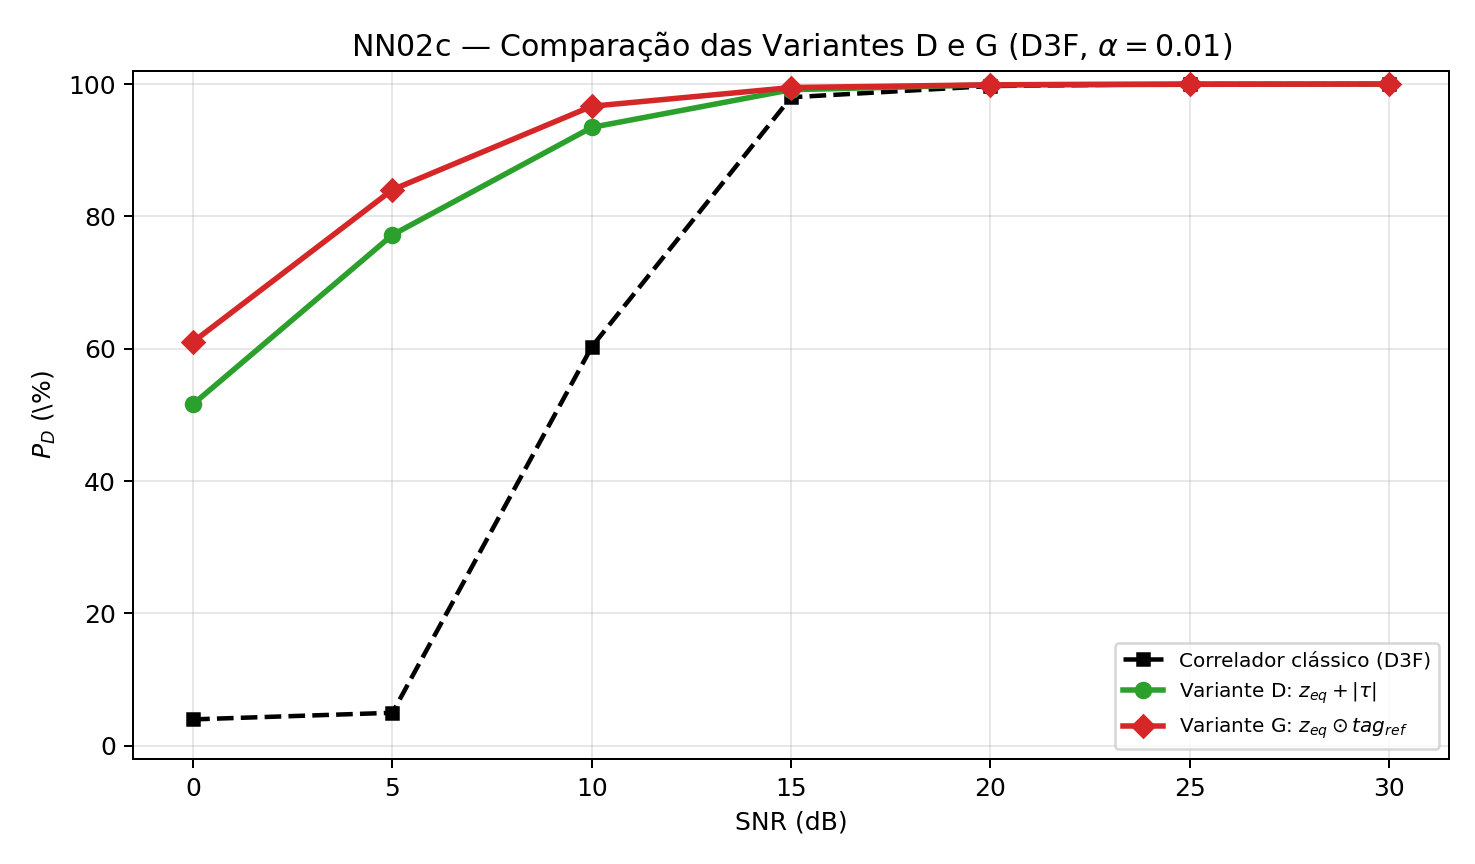
\includegraphics[width=\columnwidth]{NN02c_D_vs_G_PD_vs_SNR.png}
    \caption{\label{fig:nn02c_pd_snr}Comparação de $P_D$ versus SNR entre o correlador clássico e as Variantes D e G. A Variante D recebe $z_{eq}$ e $|\tau|$; a Variante G recebe o produto elemento a elemento $z_{eq}\odot tag_{ref}$.}
\end{figure}

\begin{figure}[htb]
    \centering
    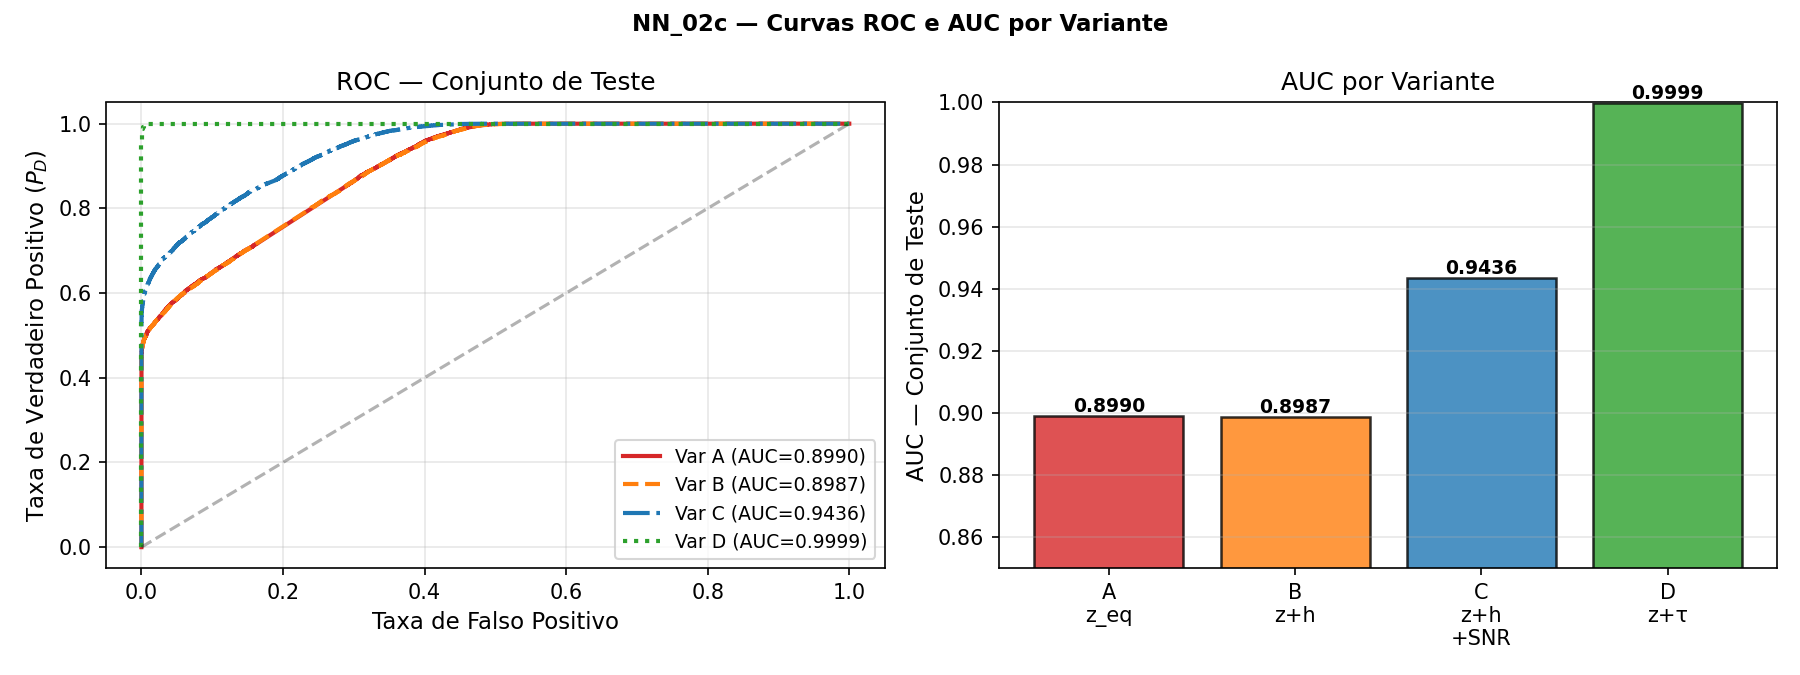
\includegraphics[width=\columnwidth]{NN_02c_ROC_AUC.png}
    \caption{\label{fig:nn02c_roc_auc}Curvas ROC/AUC complementares para comparação da separabilidade entre hipóteses nas variantes de entrada.}
\end{figure}

\section{Conclusões}\label{sec:conclusions}

Os resultados executados em NN\_02b, NN\_02c e NN\_07 confirmam três conclusões centrais. A primeira é que a representação de entrada domina o desempenho em baixo SNR. Modelos que recebem estatísticas de correlação explícitas ou preservam informação de canal superam de forma consistente a referência clássica em 0 dB. A segunda é que, no experimento final do NN\_02c, a Variante G alcança $61{,}1\%$ de detecção em 0 dB, contra $51{,}6\%$ da Variante D, indicando que a entrega ponto a ponto do produto $z_{eq}\odot tag_{ref}$ preserva informação que não está disponível quando a correlação é reduzida imediatamente a um único escalar. A terceira é que essa melhora deve ser interpretada como evidência experimental de uma representação mais adequada, e não como prova de superação do LRT teórico; D e G continuam usando limiares D3F calibrados por faixa de SNR.

A consolidação no NN\_07 confirmou que os ganhos observados nos notebooks individuais não são artefatos locais de execução, mas refletem uma tendência estável do problema: integração coerente explícita e adaptação ao canal instantâneo são os dois fatores determinantes sob restrição ultraestrita de falso alarme ($\alpha=10^{-7}$). Esses resultados sustentam a formulação do detector orientado a dados no contexto de PLA com fading Rayleigh.

Como próximos passos, o estudo pode ser estendido para cenários veiculares não estacionários, com dinâmica temporal e canais Rician, mantendo o mesmo protocolo de comparação justa entre variantes de entrada e classes de classificador. Esse avanço permitirá separar, com maior precisão, o que decorre da física do canal e o que decorre da capacidade de modelagem da arquitetura.

\section*{Agradecimentos}
Os autores agradecem ao Departamento de Eletrônica e Sistemas da Universidade Federal de Pernambuco pelo apoio na realização deste trabalho.

\section*{Lista de Siglas}
{\small
\begin{tabular}{@{}p{1.9cm}p{5.9cm}@{}}
\textbf{1D CNN}    & \textit{One-Dimensional Convolutional Neural Network} \\
\textbf{AWGN}      & \textit{Additive White Gaussian Noise} \\
\textbf{BCE}       & \textit{Binary Cross-Entropy} (Entropia Cruzada Binária) \\
\textbf{BN}        & \textit{Batch Normalization} \\
\textbf{BPSK}      & \textit{Binary Phase Shift Keying} \\
\textbf{CFAR}      & \textit{Constant False Alarm Rate} (Taxa Constante de Falso Positivo) \\
\textbf{CNN}       & \textit{Convolutional Neural Network} \\
\textbf{CSI}       & \textit{Channel State Information} \\
\textbf{D3F}       & \textit{Data-Driven Detection Framework}~\cite{ref_braca} \\
\textbf{DNN}       & \textit{Deep Neural Network} \\
\textbf{GAP}       & \textit{Global Average Pooling} \\
\textbf{IoT}       & \textit{Internet of Things} \\
\textbf{LOS}       & \textit{Line-of-Sight} \\
\textbf{LRT}       & \textit{Likelihood Ratio Test} \\
\textbf{MLE}       & \textit{Maximum Likelihood Estimation} \\
$\boldsymbol{P_D}$ & Probabilidade de Detecção \\
\textbf{PLA}       & \textit{Physical Layer Authentication} \\
\textbf{ReLU}      & \textit{Rectified Linear Unit} \\
\textbf{SNR}       & \textit{Signal-to-Noise Ratio} \\
\textbf{SVM}       & \textit{Support Vector Machine} \\
\textbf{TAG}       & Sequência de Autenticação \\
\textbf{TCL}       & Teorema Central do Limite \\
\textbf{V2X}       & \textit{Vehicle-to-Everything} \\
\end{tabular}
}

\begin{thebibliography}{99}

\bibitem{ref_sainath2015} T. N. Sainath, A. R. Mohamed, B. Kingsbury, e B. Ramabhadran, ``Convolutional, Recurrent, and Fully Connected Deep Neural Networks for Acoustic Modeling,'' em \textit{Proc.\ IEEE Int.\ Conf.\ Acoust.\ Speech Signal Process.\ (ICASSP)}, Vancouver, BC, Canadá, 2013, pp.~6645--6649.

\bibitem{ref_oshea2017} T. J. O'Shea e J. Hoydis, ``An Introduction to Deep Learning for the Physical Layer,'' \textit{IEEE Trans.\ Cogn.\ Commun.\ Netw.}, v.~3, n.~4, pp.~563--575, 2017.

\bibitem{ref_xie} H. Xie, W. Chen, e J. Ning, ``Security Model of Authentication at the Physical Layer and Performance Analysis over Fading Channels,'' \textit{IEEE Trans.\ Inf.\ Forensics Security}, v.~16, pp.~3945--3959, 2021.

\bibitem{ref_v2x_latency} 3GPP, ``3GPP TS 22.186: Enhancement of 3GPP Support for Reliable Low-Latency Communications,'' Technical Specification, v.~17.1.0, 3rd Generation Partnership Project, 2022.

\bibitem{ref_braca} P. Braca, S. Marano, V. Matta, e P. Willett, ``Statistical Hypothesis Testing Based on Machine Learning: Large Deviations Analysis,'' \textit{IEEE Open J.\ Signal Process.}, v.~3, pp.~464--484, 2022.

\bibitem{ref_liao} L. Liao, O. Wijesinghe, J. Perez-Ramirez, A. Bhatt, B. Imtiaz, e K. Ding, ``Deep Learning for Wireless Communications,'' \textit{Sensors}, v.~19, n.~11, p.~2440, 2019.

\bibitem{ref_joao} J. V. C. Evangelista, D. Moreno, D. P. B. Chaves e C. Pimentel, ``Tag Generation Using Chaotic Sequences for Physical-Layer Authentication,'' \textit{IEEE Access}, v.~11, pp.~73080--73087, 2023.

\bibitem{ref_yu} P. L. Yu, J. S. Baras, e B. M. Sadler, ``Physical-Layer Authentication,'' \textit{IEEE Trans.\ Inf.\ Forensics Security}, v.~3, n.~1, pp.~38--51, 2008.

\bibitem{ref_poor} H. V. Poor, \textit{An Introduction to Signal Detection and Estimation}, 2.~ed. Springer-Verlag, 1994.

\bibitem{ref_hash_pla} ``A Physical-Layer Authentication Scheme Based on Hash Method,'' \textit{Journal of Electronics \& Information Technology}, v.~38, n.~5, pp.~1032--1039, 2016.

\bibitem{ref_ldpc_auth} ``An LDPC Code Based Physical Layer Message Authentication Scheme with Perfect Security,'' \textit{IEEE Communications Letters}, v.~22, n.~5, pp.~954--957, 2018.

\bibitem{ref_survey_ml_pla} ``A Survey of Machine Learning-based Physical-Layer Authentication in Wireless Communications,'' arXiv:2411.09906, 2024.

\bibitem{ref_wang_dnn_csi} Q. Wang, H. Li, Z. Chen, D. Zhao, S. Ye, e J. Cai, ``Supervised and Semi-Supervised Deep Neural Networks for CSI-Based Authentication,'' arXiv:1807.09469, 2018.

\bibitem{ref_comparison_stat_ml} ``Comparison of Statistical and Machine Learning Techniques for Physical Layer Authentication,'' arXiv:2001.06238, 2020.

\bibitem{ref_clustering_pla} ``Clustering Based Physical-Layer Authentication in Edge Computing Systems with Asymmetric Resources,'' \textit{Sensors}, v.~19, n.~8, 2020.

\bibitem{ref_biometric_chaotic} ``Physical Layer Authenticated Image Encryption for IoT Network Based on Biometric Chaotic Signature for MPFrFT OFDM System,'' \textit{Sensors}, v.~23, n.~18, p.~7843, 2023.

\bibitem{ref_transformer_csi_pred} ``Channel Prediction-Based Physical Layer Authentication under Consecutive Spoofing Attacks,'' arXiv:2603.19962, 2026.

\bibitem{ref_adam} D. P. Kingma e J. Ba, ``Adam: A Method for Stochastic Optimization,'' em \textit{Proc.\ Int.\ Conf.\ Learn.\ Represent.\ (ICLR)}, San Diego, CA, EUA, 2015.

\bibitem{ref_goodfellow} I. Goodfellow, Y. Bengio e A. Courville, \textit{Deep Learning}. MIT Press, 2016.

\bibitem{ref_proakis} J. G. Proakis e D. G. Manolakis, \textit{Digital Signal Processing: Principles, Algorithms, and Applications}, 4.~ed. Pearson Prentice Hall, 2007.

\bibitem{ref_3gpp} 3GPP, ``Study on Channel Model for Frequencies from 0.5 to 100 GHz,'' Technical Report TR 38.901, v.~17.0.0, 3rd Generation Partnership Project, 2022.

\bibitem{ref_shlezinger} N. Shlezinger, N. Farsad, Y.~C. Eldar e A.~J. Goldsmith, ``Model-Based Machine Learning for Communications,'' arXiv:2101.04726, 2021.

\bibitem{ref_veldhuis} R. Veldhuis e D. Zeng, ``On Neyman-Pearson Optimality of Binary Neural Net Classifiers,'' Tech.\ Rep., jun.\ 2021. DOI: 10.36227/techrxiv.14709930.v1.

\bibitem{ref_kay} S. M. Kay, \textit{Fundamentals of Statistical Signal Processing, Vol.~I: Estimation Theory}. Prentice Hall, 1993.

\bibitem{ref_raya} M. Raya e J.-P. Hubaux, ``Securing Vehicular Ad Hoc Networks,'' \textit{J. Comput. Secur.}, v.~15, n.~1, pp.~39--68, 2007.

\bibitem{ref_digham} F. F. Digham, M.-S. Alouini e M. K. Simon, ``On the Energy Detection of Unknown Signals Over Fading Channels,'' \textit{IEEE Trans.\ Commun.}, v.~55, n.~1, pp.~21--24, Jan.\ 2007.

\end{thebibliography}

\end{document}
